\documentclass[pdf,dvipsnames]{beamer}
% \usetheme{Antibes}
\usetheme{Frankfurt}

\usepackage{xkeyval}
\usepackage{todonotes}
\presetkeys{todonotes}{inline}{}
\usepackage{graphicx}
\usepackage{subfig}
\usepackage{multimedia}                % include movies
\usepackage{breqn}                     % break equations automatically
\usepackage{cancel}                    % cancel out text/equations
\usepackage{color}                     % colored font
\usepackage{wasysym}                   % smiley (smiling face)
\usepackage[absolute,overlay]{textpos} % to put a box in front of text
\usepackage{mathtools}                 % use dcases to display nice fractions in cases
\usepackage{multicol}                  % split tof
\usepackage[figurename=Fig]{caption}
\usepackage{tcolorbox}
\usepackage{calc}
\usepackage{multirow}
\usepackage{dcolumn}
\usepackage{adjustbox}

\usepackage{hyperref}
\hypersetup{
	pdftitle   = {Brown bag seminar},
	pdfauthor  = {Pablo Botas},
	pdfcreator = {Pablo Botas},
	colorlinks = true,
	linkcolor  = cyan,
	linktoc    = black,
	citecolor  = black,
	filecolor  = black,
	urlcolor   = black,
	baseurl={}
}

\setlength\abovecaptionskip{0pt}

\usepackage{pgfpages}
% \setbeameroption{show notes on second screen}
\beamertemplatenavigationsymbolsempty
\setbeamertemplate{footline}[frame number]

\newcommand\blfootnote[1]{%
	\begingroup
	\renewcommand\thefootnote{}\footnote{#1}%
	\addtocounter{footnote}{-1}%
	\endgroup
}

% SEE http://latexcolor.com/
\definecolor{flame}{rgb}{0.89, 0.35, 0.13}
\definecolor{iceberg}{rgb}{0.44, 0.65, 0.82}
\definecolor{inchworm}{rgb}{0.7, 0.93, 0.36}
\definecolor{brandeisblue}{rgb}{0.0, 0.44, 1.0}

\AtBeginDocument{\setlength\abovedisplayskip{0pt}}
\AtBeginDocument{\setlength\belowdisplayskip{10pt}}
\AtBeginDocument{\setlength\abovedisplayshortskip{0pt}}
\AtBeginDocument{\setlength\belowdisplayshortskip{0pt}}


\begin{document}
\title{Online adaptation of IMPT plans with GPU-MC dose calculation on CBCTs for head and neck}
\subtitle{Brown bag seminar}
\institute{Massachusetts General Hospital and Heidelberg University}
\titlegraphic{
	
\includegraphics[height=2cm]{imgs/MGHHMSLogo.pdf} \hspace*{2cm} ~%
	
\includegraphics[height=2cm]{imgs/Logo_University_of_Heidelberg.pdf}
}
\date{May 1, 2017}
\begin{frame}
    \titlepage
    \note{I am going to present a study that we recently finished of what can be done to limit the plan degradation for mobile lung cancer tumors. However, I'll to start with the subtitle, I know of some people in the department interested in implementing this tool in the clinical routines so I am going to introduce how it works and what steps are followed. I will keep this as brief as possible because it's not necessarily translatable to the clinic.}
\end{frame}

\begin{frame}{General outline}
    \begin{multicols}{2}
        \tableofcontents[sectionstyle=show,
                         subsectionstyle=show/show,
                         subsubsectionstyle=show/show,
                         subsubsectionstyle=show/show/show]
    \end{multicols}
\end{frame}

%\begin{frame}{Comments given after the talk}
%    \begin{multicols}{2}
%        \todo{Since you are overwritting the density and MC is more sensitive to it, would this create worse plans? This is a tricky issue.}
%        \todo{You have shown that WEPL is superior for these cases. Wouldn't the others be more robust?}
%    \end{multicols}
%\end{frame}

\section{Introduction}

%****************New Frame******************
\begin{frame}[c]{Why is online adaptation needed?}
    Being the ultimate goal to better conform dose to the target\ldots
    \begin{itemize}
        \item<1-> \textbf{Setup} uncertainties
        \item<1-> Patient \textbf{anatomy} inter-fractional variation
        \item<2-> Protons are sensitive to geometry changes
        \item<2-> Target \textbf{coverage} may be compromised
        \item<3-> Security \textbf{margins} increase high dose region
        \item<4-> Higher dose to \textbf{OARs}
        \item<5-> A risky statement: \textbf{Robust planning} can not cover every possible scenario and increases high dose volume
    \end{itemize}
    \onslide<6->{
        \begin{exampleblock}{}
            Online adaptation would allow margin reduction guaranteeing coverage and OAR sparing at before every fraction is delivered
        \end{exampleblock}
    }
\end{frame}


\begin{frame}[c]{The Head and Neck case}
    \begin{columns}[c]
        \begin{column}[c]{0.45\textwidth}
            \begin{figure}[h]
                \centering
                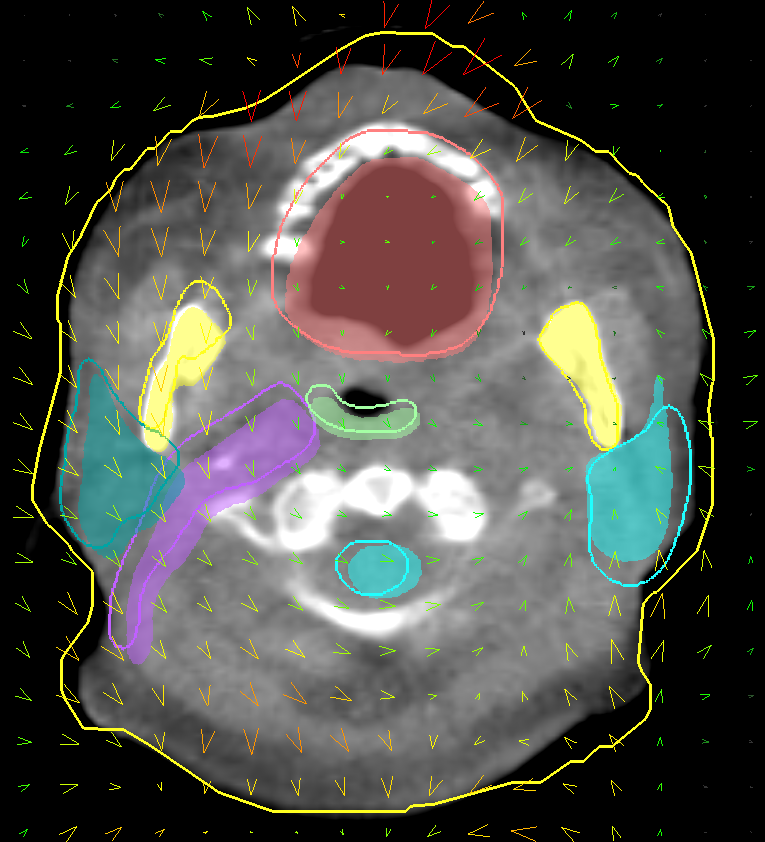
\includegraphics[width=\textwidth]{imgs/patient_deformation.png}
                \caption{Head and neck patient geometry changes. The arrows represent the vector field.}
            \end{figure}
        \end{column}
        \begin{column}{0.55\textwidth}
            \textbf{Potential for increased treatment quality:}
            \begin{itemize}
                \item OARs very close to the target
                \item Large inter-fractional anatomy changes
                \item Tissue interfaces make it sensitive
            \end{itemize}
        \end{column}
    \end{columns}
\end{frame}

\section{Objectives}
\begin{frame}[c]{Objectives:}
	Aim: Change the IMPT fields to recover initial plan quality while the patient is on the couch
	
    Goals:
    \begin{itemize}
    	\item Develop an \textbf{online} adaptation algorithm
    	\item Dose calculations with GPU-MC on CBCTs
    \end{itemize}
    \pause
    Steps:
    \begin{itemize}
        \item Plan set of patients with IMPT and no margin on CTV
        \item Study plan evolution \textit{vs} anatomy changes on CBCT images
        \item Can we get away with plan adjustments as opposed to replanning?
    \end{itemize}
\end{frame}

\begin{frame}[c]{What has been published?}
	\begin{columns}[c]
		\column{0.5\textwidth}
		\begin{block}{Kurz 2016}
			\begin{itemize}
				\item Offline
				\item Analytical dose calculation
				\item Full reoptimization
				\item Adaptation on vCT
			\end{itemize}
		\end{block}
		\begin{block}{Moriya 2017}
			\begin{itemize}
				\item Range shifter of the day
				\item Passive scattering for lung
			\end{itemize}
		\end{block}
		\column{0.5\textwidth}
		\begin{block}{Jagt 2017}
			\begin{itemize}
				\item Online (more or less)
				\item Analytical dose calculation
				\item Dose restoration
				\item Full reoptimization
				\item Original contours
			\end{itemize}
		\end{block}
		\begin{block}{Bernatowitz 2018}
			\begin{itemize}
				\item Extension of \textit{Jagt et al.} for robust optimization and others
			\end{itemize}
		\end{block}
	\end{columns}
\end{frame}






\begin{frame}{General outline}
	\begin{multicols}{2}
		\tableofcontents[sectionstyle=show,
		subsectionstyle=show/show,
		subsubsectionstyle=show/show,
		subsubsectionstyle=show/show/show]
	\end{multicols}
\end{frame}

\section{Methods}

\begin{frame}[c]{Traditional workflow:}
    \begin{overprint}
    \onslide<1>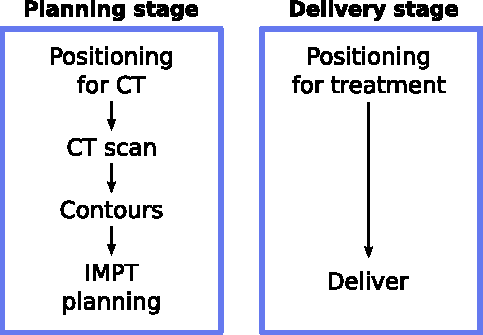
\includegraphics[scale=0.86]{imgs/workflow_trad_1.pdf}
    \onslide<2>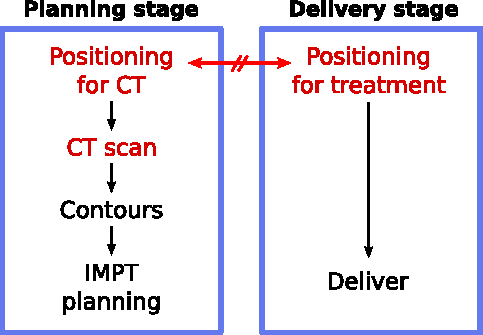
\includegraphics[scale=0.86]{imgs/workflow_trad_2.pdf}
    \end{overprint}
\end{frame}

\begin{frame}[c]{Patient cohort planned without margin around CTV}
	\begin{table}[h]
		\scalebox{0.7}{
			\begin{tabular}{ccp{1cm}|p{1cm}p{2.5cm}|p{3cm}p{3cm}}
				\hline
				Pat. No. & Location & No. beams & No. CBCTs & Plan CTV vol. ($cm^3$) & Average CTV vol. ratio (min, max) & Average CTV dice (min, max) \\
				\hline
				1 & Oropharynx & 4 & 6 & 22.3 & 1.00 (0.97, 1.05) & 0.58 (0.50, 0.67) \\
				2 & Tonsil & 2 & 6 & 9.0 & 1.02 (0.94, 1.12) & 0.87 (0.83, 0.90) \\
				3 & Oropharynx & 3 & 7 & 30.7 & 0.93 (0.90, 1.00) & 0.82 (0.77, 0.88) \\
				4 & Neck & 4 & 6 & 81.3 & 1.03 (0.98, 1.06) & 0.79 (0.75, 0.84) \\
				5 & Hypopharynx & 3 & 5 & 59.6 & 0.97 (0.95, 0.98) & 0.89 (0.87, 0.91) \\
				6 & Mouth & 3 & 7 & 116.5 & 0.78 (0.75, 0.82) & 0.87 (0.83, 0.90) \\
				7 & Larynx & 3 & 6 & 25.0 & 1.21 (1.08, 1.34) & 0.84 (0.77, 0.88) \\
				8 & Tongue & 4 & 5 & 79.9 & 1.06 (1.04, 1.11) & 0.87 (0.82, 0.91) \\
				9 & Tonsil & 2 & 6 & 12.0 & 0.98 (0.95, 1.00) & 0.87 (0.83, 0.93) \\
				10 & Oropharynx & 3 & 7 & 95.9 & 0.96 (0.91, 1.02) & 0.89 (0.85, 0.92) \\
				\hline
				Summary: & - & - & 61 & 63.22 $\pm$ 45.1 & 0.98 $\pm$ 0.11 & 0.83 $\pm$ 0.09 \\
				\hline \\
			\end{tabular}}
			\caption{Patient cohort summary}
		\end{table}
	\end{frame}

\begin{frame}[c]{What are we facing?}
    \begin{columns}[c]
        \column[c]{0.45\textwidth}
        \begin{figure}[h]
            \centering
            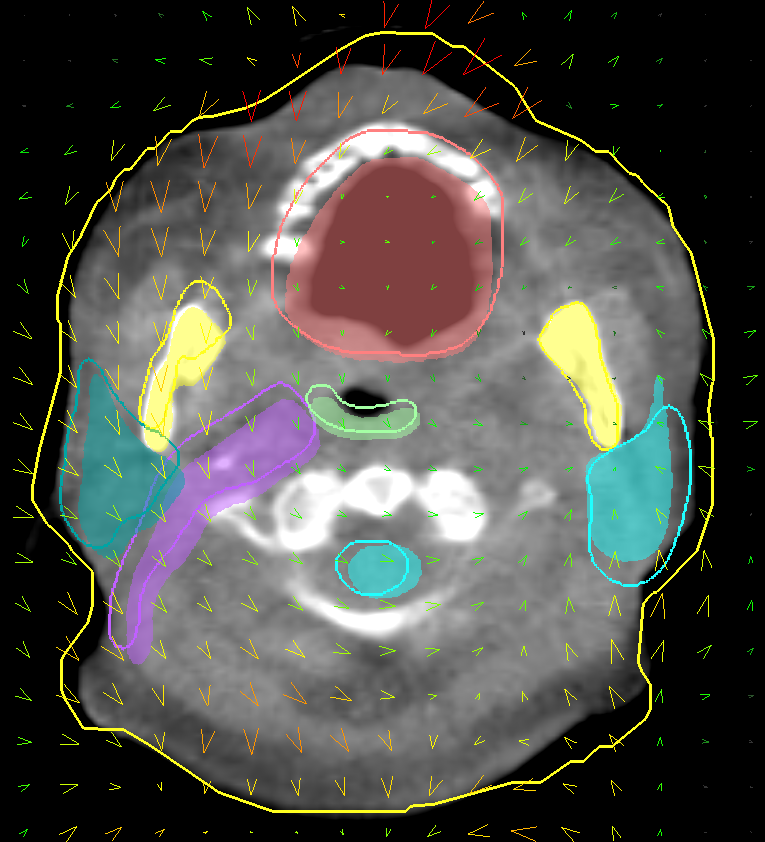
\includegraphics[width=\textwidth]{imgs/patient_deformation.png}
            \caption{Head and neck patient geometry changes. The arrows represent the vector field.}
        \end{figure}
        \column[c]{0.55\textwidth}
        \onslide<2>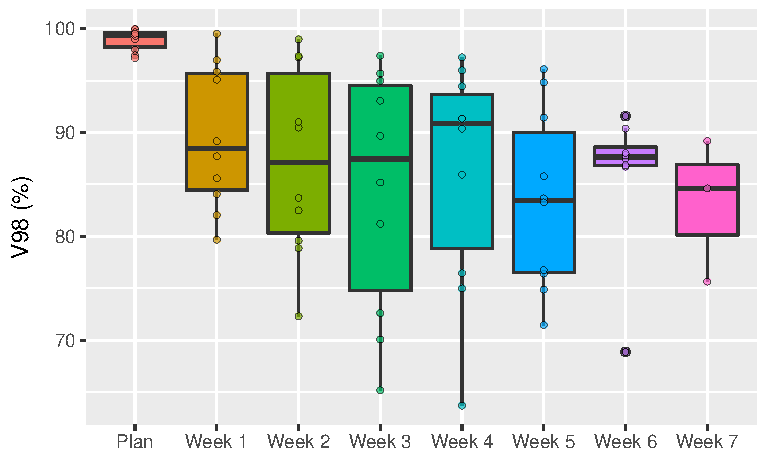
\includegraphics[width=\textwidth]{imgs/plan_evolution_V98.pdf}\\
        \onslide<2>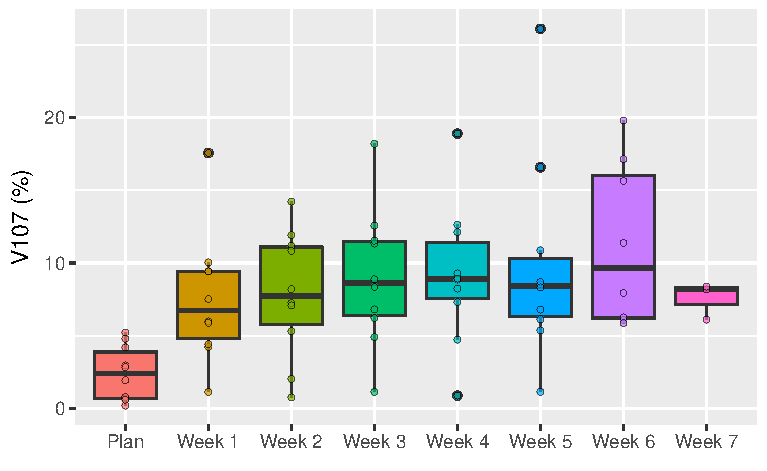
\includegraphics[width=\textwidth]{imgs/plan_evolution_V107.pdf}
    \end{columns}
\end{frame}

\begin{frame}[c]{Traditional workflow:}
    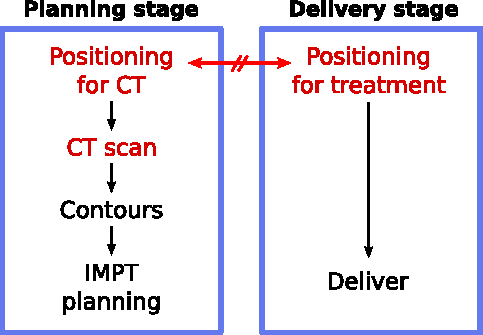
\includegraphics[scale=0.86]{imgs/workflow_trad_2.pdf}
\end{frame}

\begin{frame}[c]{Adaptation workflow:}
    \begin{overprint}
    \onslide<1>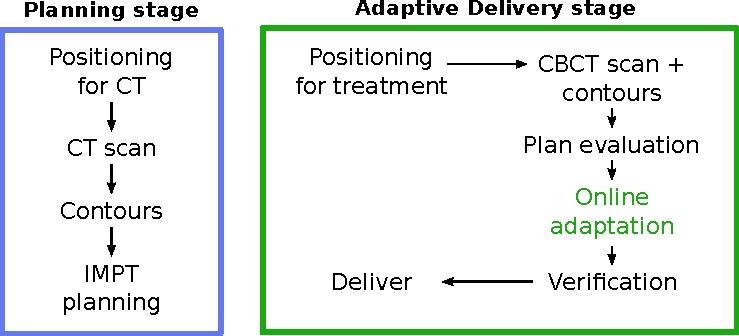
\includegraphics[scale=0.86]{imgs/workflow_adaptive_1.pdf}
    \onslide<2>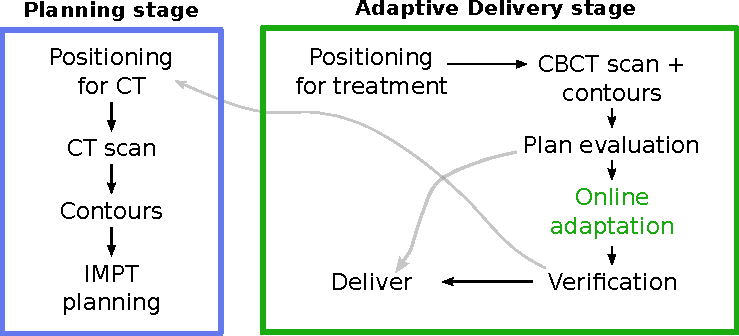
\includegraphics[scale=0.86]{imgs/workflow_adaptive_2.pdf}
    \end{overprint}
\end{frame}

\begin{frame}[c]{Necessary tools}
	\begin{columns}[t]
		\begin{column}{0.5\textwidth}
        {\setbeamercolor{block title}{bg=flame, fg=black}
        \begin{block}{Cone Beam CT (CBCT)}
            \textit{A priori} CT-based scatter correction WEPL error $< 2\%$ in head cases.\\
            {\begin{flushright}\scriptsize\textit{Park et al., Med Phys. 2015;42(8)}, \textit{Kim et al., Phys Med Bio. 2017;62(1)}\end{flushright}}
        \end{block}}
        {\setbeamercolor{block title}{bg=inchworm, fg=black}
        \begin{block}{Fast GPU MC: gPMC}
            Accurate dose calculation engine.\\
            {\hfill\scriptsize\textit{Qin et al., Phys Med Biol. 2016;61(20)}}
        \end{block}}
		\end{column}
		\begin{column}{0.5\textwidth}
			{\setbeamercolor{block title}{bg=iceberg, fg=black}
            \begin{block}{Image Registration: Plastimatch}
                Register planning CT to CBCT. Rigid and deformable (DIR), GPU B-spline\\
                {\hfill\scriptsize\textit{Shackleford et al., Phys Med Biol. 2010;55(21)}}
            \end{block}}
            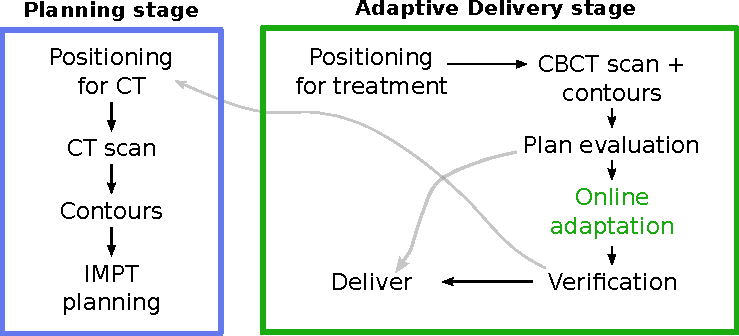
\includegraphics[width=\textwidth]{imgs/workflow_adaptive_2.pdf}
		\end{column}
	\end{columns}
\end{frame}


\begin{frame}[c]{Adaptation steps}
    Adaptation steps:
    \begin{enumerate}
        \item \textbf{Geometrical adaptation:} spots are moved following a VF and the energy is adjusted after raytracing
        \item \textbf{Weight adaptation:} tune spot weights to correct for the unbalance created by the geometrical adaptation
    \end{enumerate}
    \pause
    Why does this study not include setup uncertainties and what does it mean?
\end{frame}


\begin{frame}[c]{Geometrical adaptation: basics}
	\begin{columns}[t]
		\begin{column}{0.55\textwidth}
            Per spot $s_i = (x_0, y_0, E_0)$:
            \begin{itemize}
                \item[1:]<2-> \textbf{Raytrace} $s_i$ in CT ($r_i$)
                \item[2:]<3-> \textbf{Probe} VF at $r_i$ coords: $v_i$
                \item[3:]<4-> \textbf{Apply $v_i$ to $r_i$} coords: position where the $r_i$ should be in the CBCT
                \item[4:]<5-> \textbf{Apply $v_i$ to $s$} $\rightarrow $ $s'_i = (x_0 + \Delta v_x, y_0 + \Delta v_y, E_0)_i$
                \item[5:]<6-> \textbf{Raytrace} $s'_i$ in CBCT
                \item[6:]<7-> \textbf{Get} $\Delta E_i$
            \end{itemize}
            \only<8>{Spot adaptation: $(\Delta v_x, \Delta v_y, \Delta E)_i$}
		\end{column}
		\begin{column}{0.45\textwidth}
			\vspace{-1cm}
			\begin{figure}
                \only<1>{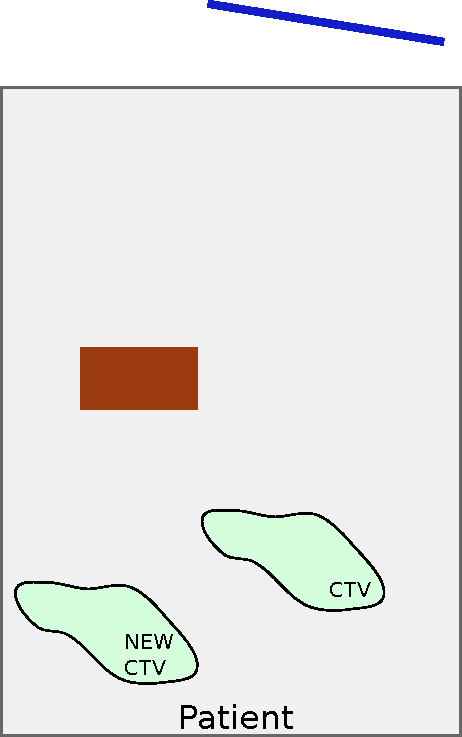
\includegraphics[height=0.8\textheight]{imgs/adaptation_method_0.pdf}}
                \only<2>{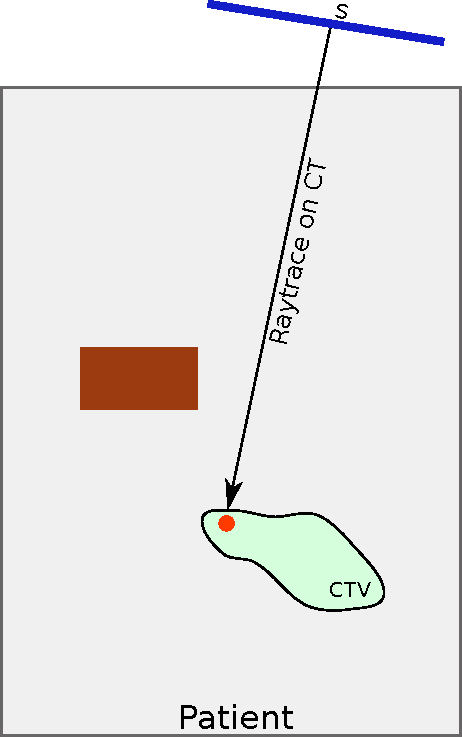
\includegraphics[height=0.8\textheight]{imgs/adaptation_method_1.pdf}}
				\only<3>{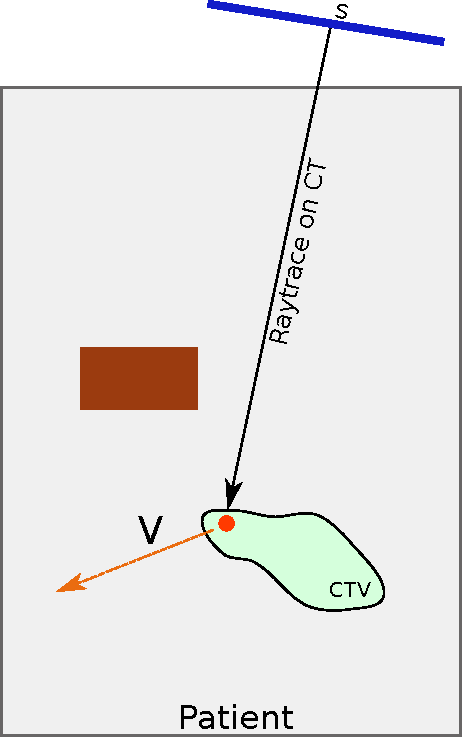
\includegraphics[height=0.8\textheight]{imgs/adaptation_method_2.pdf}}
				\only<4>{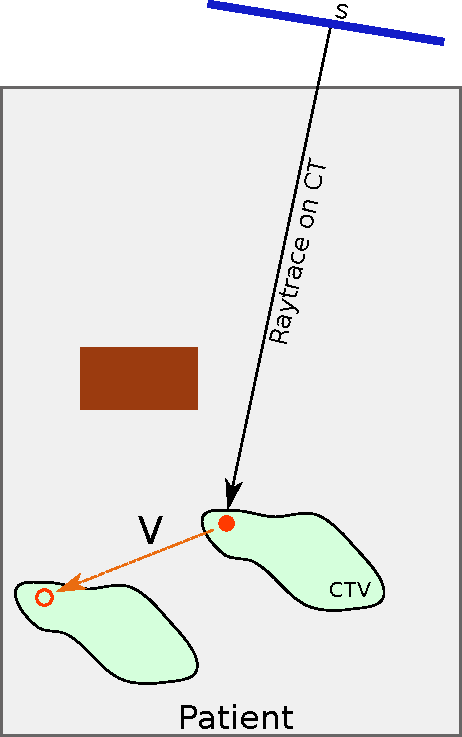
\includegraphics[height=0.8\textheight]{imgs/adaptation_method_3.pdf}}
				\only<5>{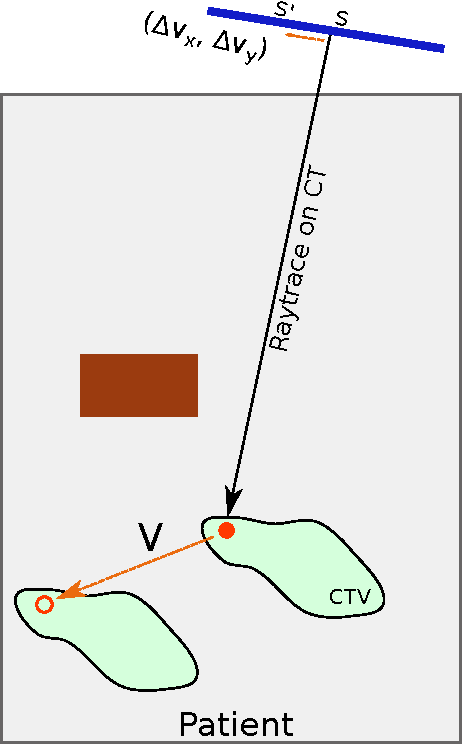
\includegraphics[height=0.8\textheight]{imgs/adaptation_method_4.pdf}}
				\only<6>{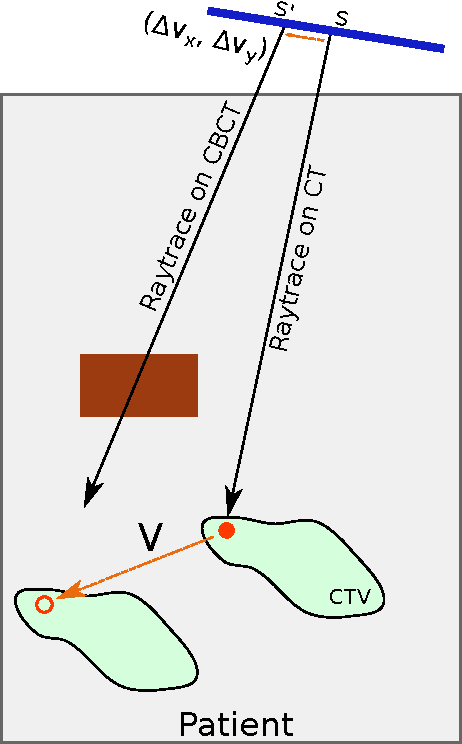
\includegraphics[height=0.8\textheight]{imgs/adaptation_method_5.pdf}}
				\only<7->{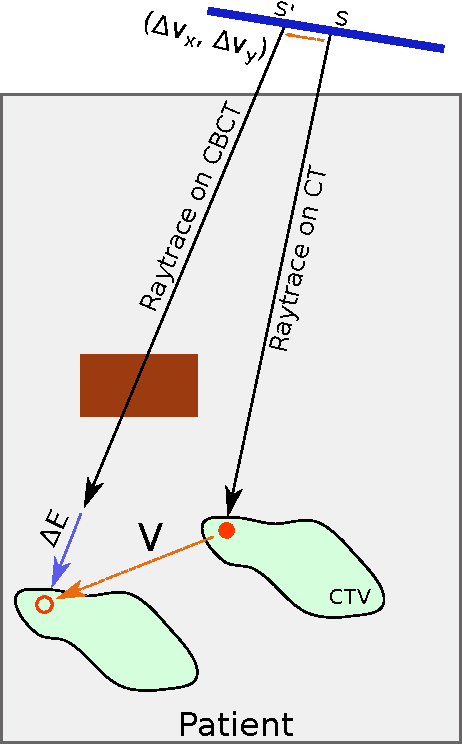
\includegraphics[height=0.8\textheight]{imgs/adaptation_method_end.pdf}}
			\end{figure}
		\end{column}
	\end{columns}
\end{frame}


\begin{frame}[c]{Geometrical adaptation: constraints}
    \begin{columns}[c]
        \begin{column}{0.45\textwidth}
            Constraints:
            \begin{itemize}
                \item {\color{brandeisblue} Free:} No constraints on spots movement $(\Delta v_x, \Delta v_y, \Delta E)_i$
                \item {\color{brandeisblue} Constrained:}
                \begin{itemize}
                    \item \textit{Couch/isocenter shift}: Average VF in the CTV
                    \item \textit{Range-shifter-of-the-day}: Average energy shift
                    \item \textit{Both}
                \end{itemize}
            \end{itemize}
        \end{column}
        \begin{column}{0.55\textwidth}
            \vspace*{-0.4cm}
            \begin{figure}[b!]
                \centering
                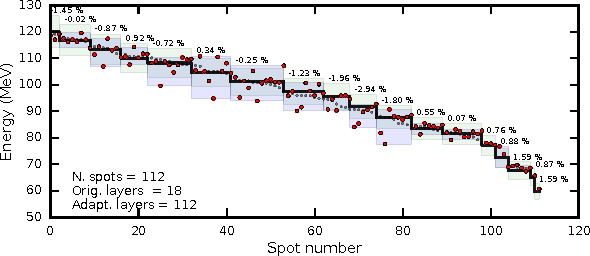
\includegraphics[width=\textwidth]{imgs/plan_energy_layer_destruction.pdf}\\
                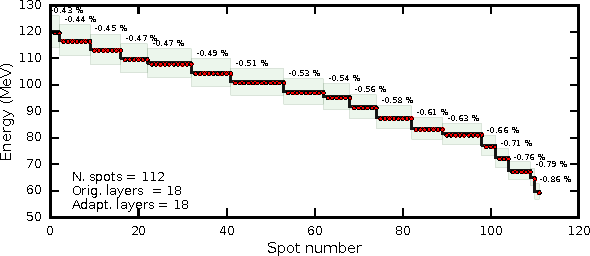
\includegraphics[width=\textwidth]{imgs/plan_energy_layer_conservation.pdf}
                \caption{Distortion and conservation of plan energy layers}
            \end{figure}
        \end{column}
    \end{columns}
\end{frame}


\begin{frame}[c]{Weight tuning:}
     Taking the proposed workflow into account\ldots
	\begin{figure}[h]
		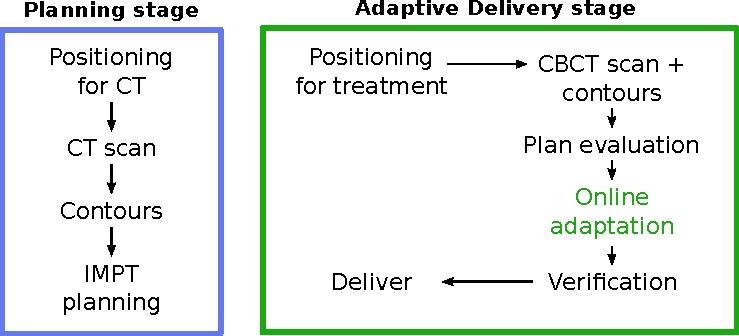
\includegraphics[scale=0.7]{imgs/workflow_adaptive_1.pdf}
	\end{figure}
    How can we gather significant information of individual spots \textbf{fast}?
\end{frame}


\begin{frame}[c]{Adaptation workflow:}
	\textbf{Use information from the initial plan: on average, 8.2\% of the spots deliver at least 50\% of the dose}
	\pause
	
	Weight tuning:
    \begin{enumerate}
    	\item Run the \textbf{geometrical adaptation} with gPMC
    	\item Define \textbf{region of interest} during simulation
    	\item Score the \textbf{dose per spot} in ROI
    	\item \textbf{Select set} of spots giving 50\% of the dose, being at least 10\% of the total spots
    	\item Accumulate adapted dose without the set
    	\item Calculate \textbf{remaining dose} for coverage in target
    	\item \textbf{Tune set weights} to fill the remaining dose with Opt4D
    \end{enumerate}
\end{frame}


\begin{frame}{General outline}
	\begin{multicols}{2}
		\tableofcontents[sectionstyle=show,
		subsectionstyle=show/show,
		subsubsectionstyle=show/show,
		subsubsectionstyle=show/show/show]
	\end{multicols}
\end{frame}


\section{Results}

\begin{frame}[c]{What does the deformation look like?}
	\begin{figure}[h]
		\centering
		\only<1>{
			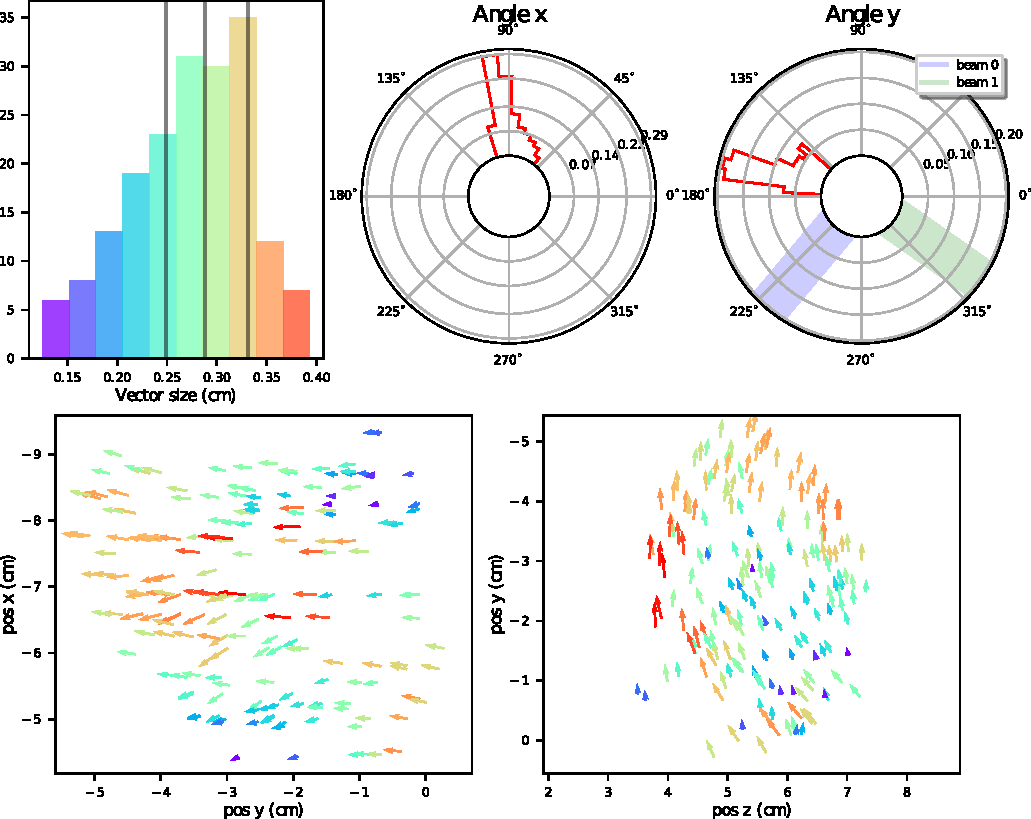
\includegraphics[height=0.8\textheight]{imgs/P015_cbct1_vf.pdf}
			\caption{Deformation field of patient 9, fraction 1}
		}
		\only<2>{
			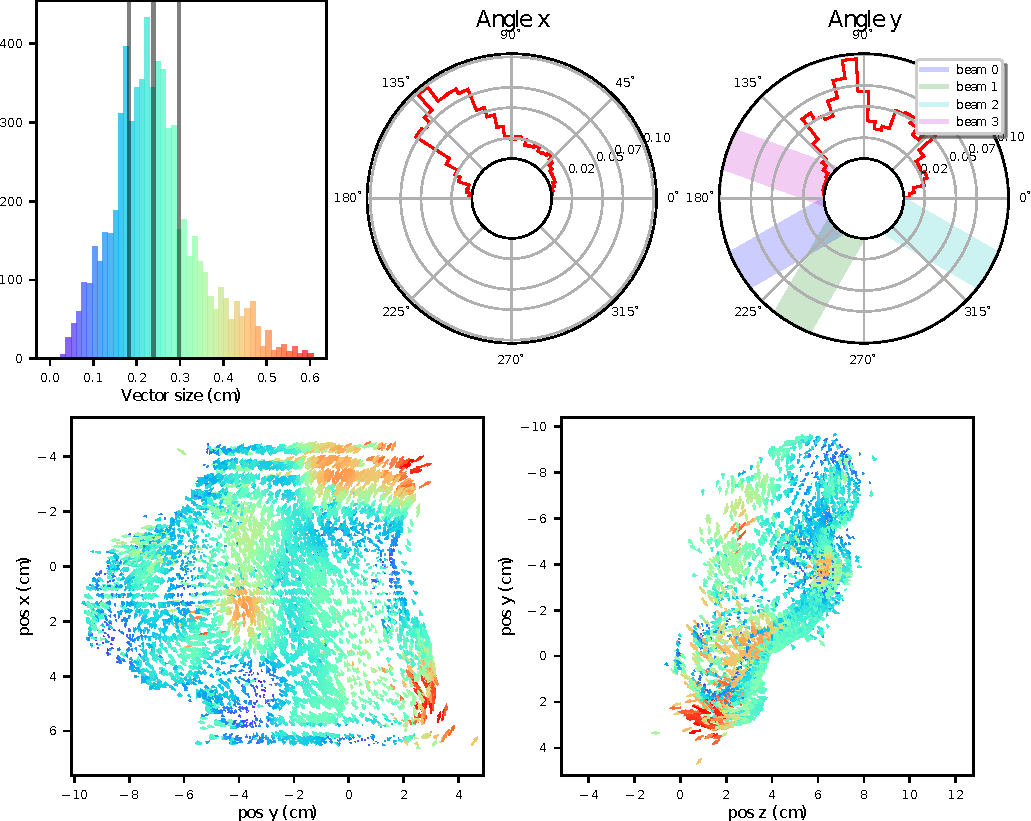
\includegraphics[height=0.8\textheight]{imgs/P04_cbct1_vf.pdf}
			\caption{Deformation field of patient 4, fraction 1}
		}
	\end{figure}
	
\end{frame}

\begin{frame}[c]{How do the spot parameters change?}
	\centering
	\only<1>{
		\begin{figure}[h]
			\centering
			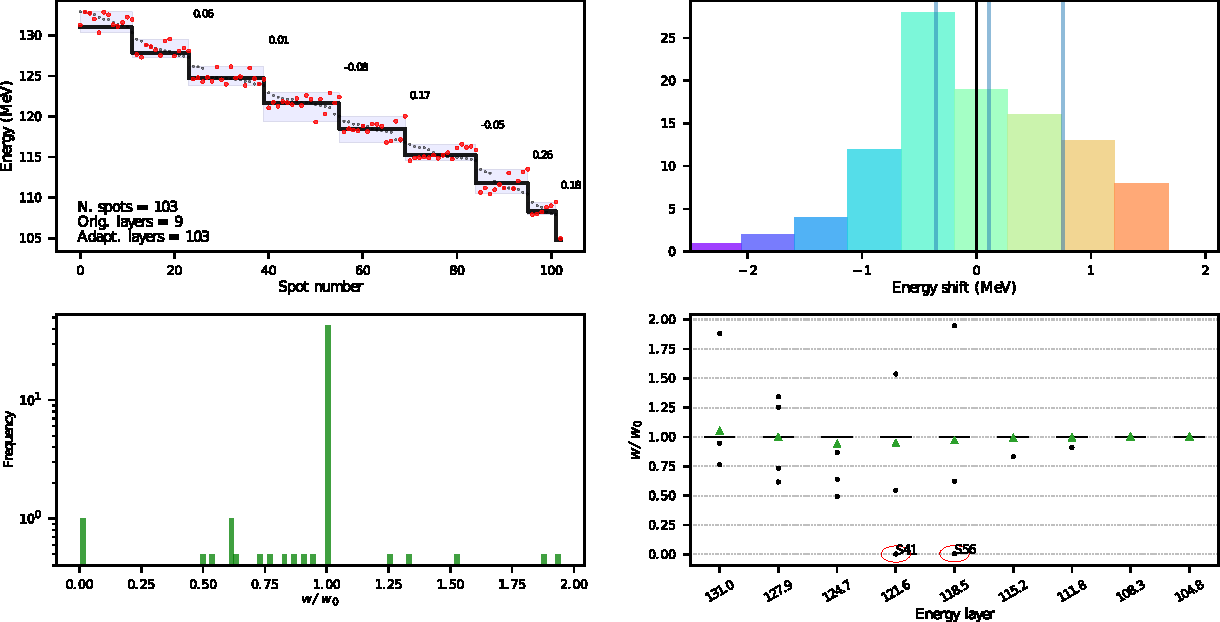
\includegraphics[width=\textwidth]{imgs/tramp_P02_cbct1.pdf}
			\caption{Fluence map changes: Patient 2, fraction 1, beam 1}
		\end{figure}
	}
	\only<2>{
		\begin{figure}[h]
			\centering
			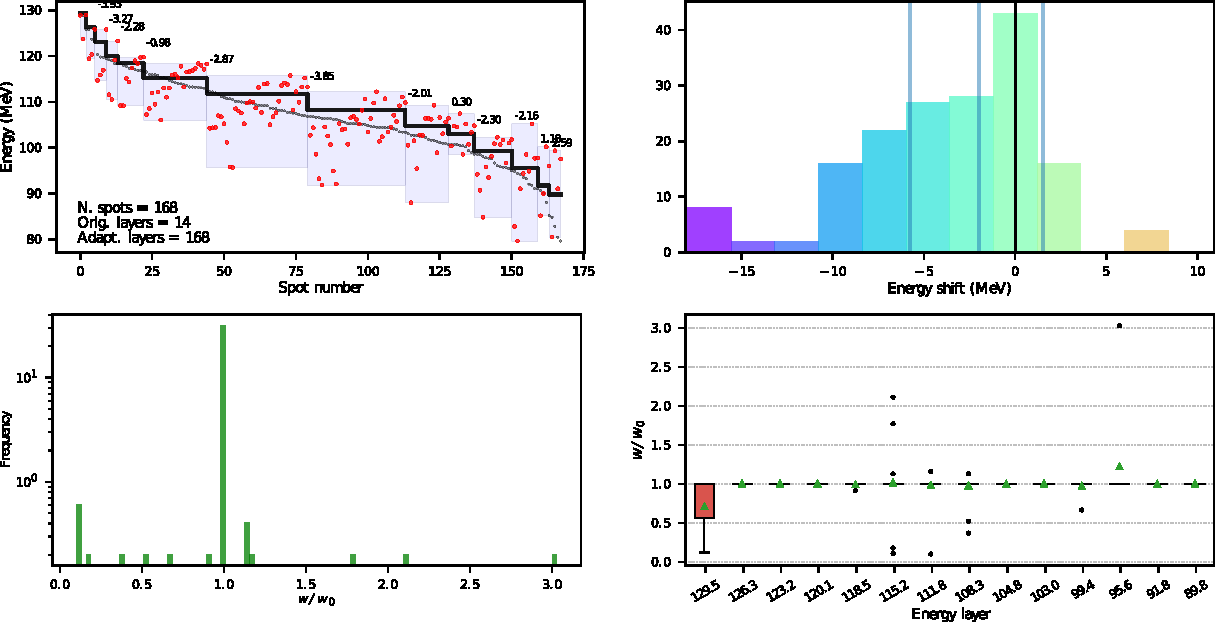
\includegraphics[width=\textwidth]{imgs/tramp_P10_cbct4.pdf}
			\caption{Fluence map changes: Patient 7, fraction 4, beam 2}
		\end{figure}
	}
\end{frame}


\begin{frame}[c]{Results: what has not worked}
	Geometric-only approaches:
	\begin{columns}[c]
		\begin{column}{0.55\textwidth}
			\begin{itemize}
				\item Not in the general case
				\item Divergences in the VF
				\item Bragg peaks changes
			\end{itemize}
		\end{column}
		\begin{column}{0.45\textwidth}
			\begin{itemize}
				\item Unbalance of spot doses
				\item Under-represented areas
				\item Constraints too strict
			\end{itemize}
		\end{column}
	\end{columns}
    \begin{figure}
        \only<2>{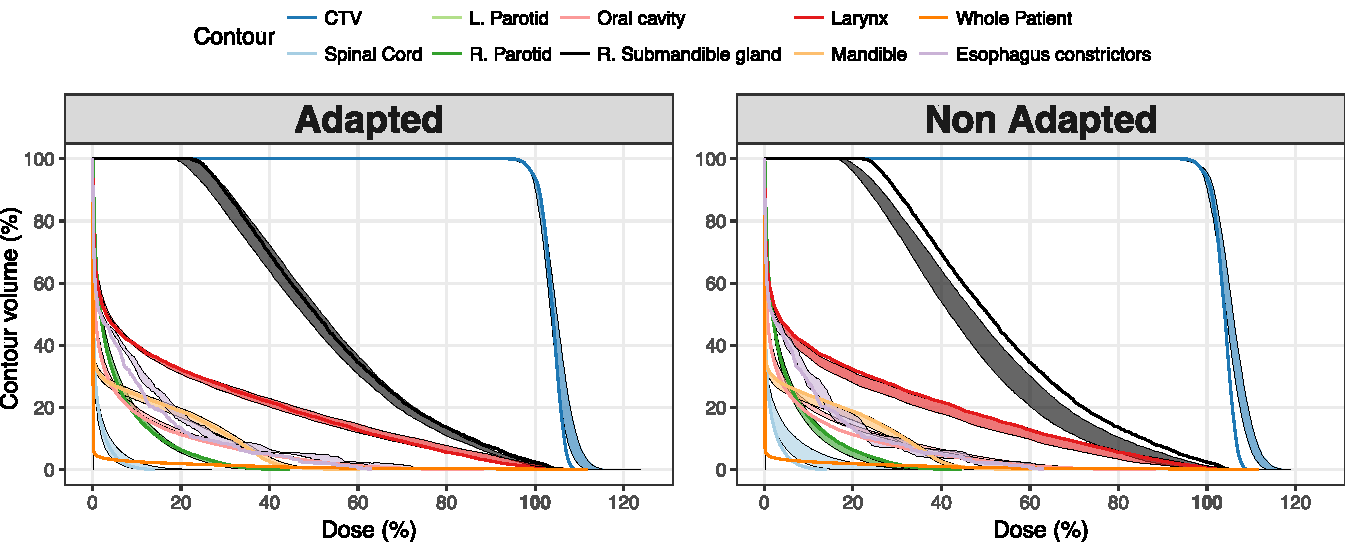
\includegraphics[width=\textwidth]{imgs/DVHs_normalized_Geo_free_P15_not_week6.pdf}}
        \onslide<3>{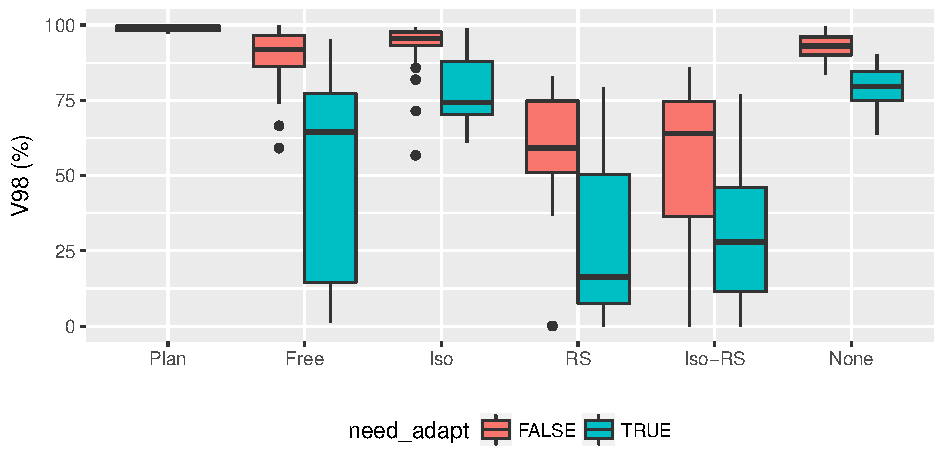
\includegraphics[width=0.9\textwidth]{imgs/target_V98_geometric_need_adapt.pdf}}
    \end{figure}
\end{frame}


\begin{frame}[c]{Results with weight tuning: CTV}
	Adjusting the weights shows improved results:
	\begin{figure}
        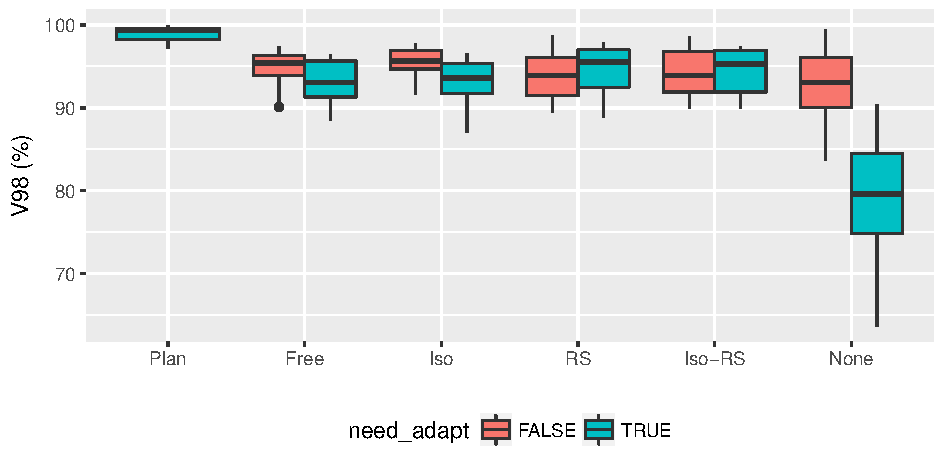
\includegraphics[width=\textwidth]{imgs/target_V98_weights_need_adapt.pdf}
    \end{figure}
    \onslide<2>{\textbf{Which one is better? Normalize and check homogeneity!!}}
\end{frame}


\begin{frame}[c]{Results with weight tuning: CTV}
    Normalized to V98 = 98\%:
    \begin{figure}
        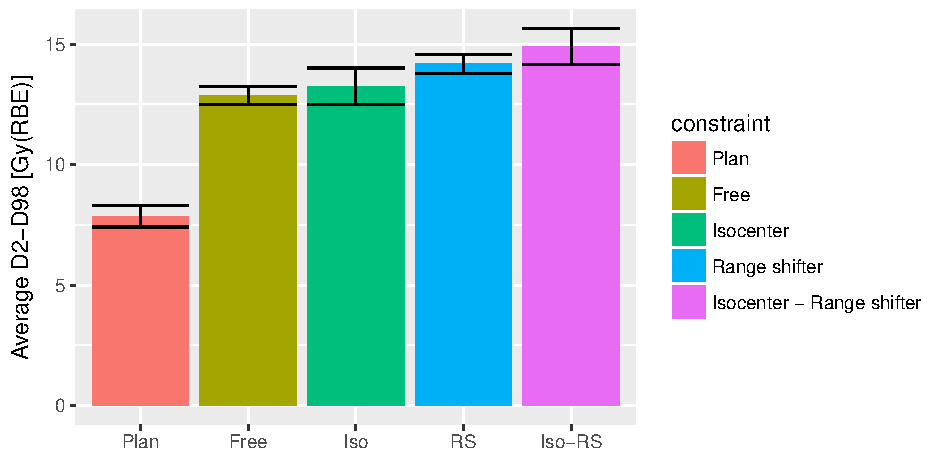
\includegraphics[width=\textwidth]{imgs/target_D2_D98_weights_comparison.pdf}
    \end{figure}
    \ldots~hard to tell between \textit{Free} and \textit{Isocenter shift}. Maybe the OARs show a clearer pattern?
\end{frame}


\begin{frame}[c]{Results with weight tuning: OARs}
	The free strategy \textit{seems} slightly better than the isocenter strategy.
	\begin{figure}
		\only<1>{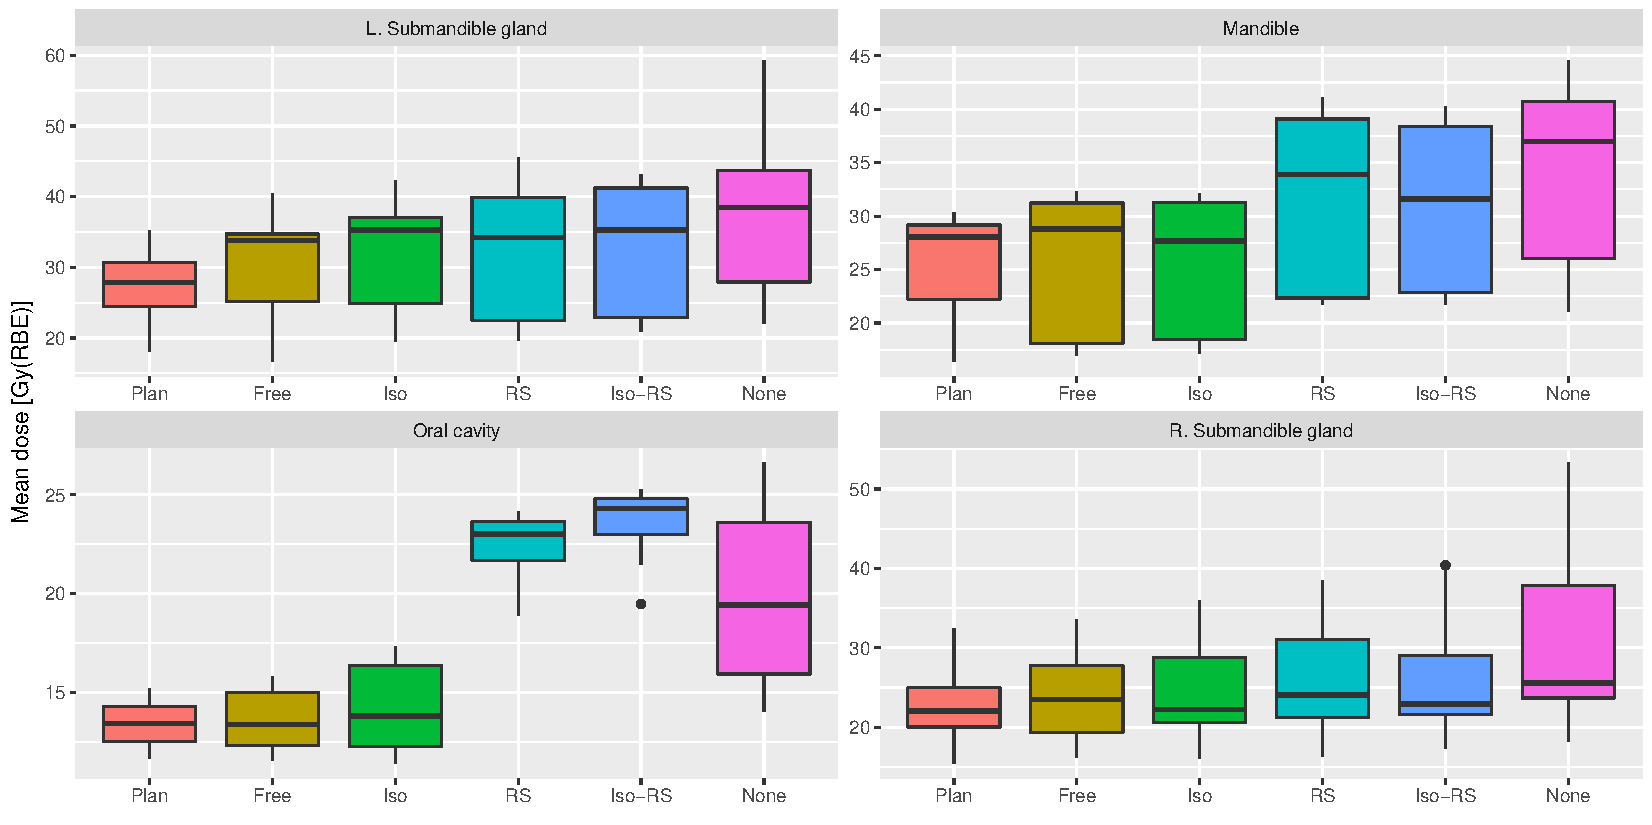
\includegraphics[width=\textwidth]{imgs/oars_mean_weights.pdf}}
		\only<2>{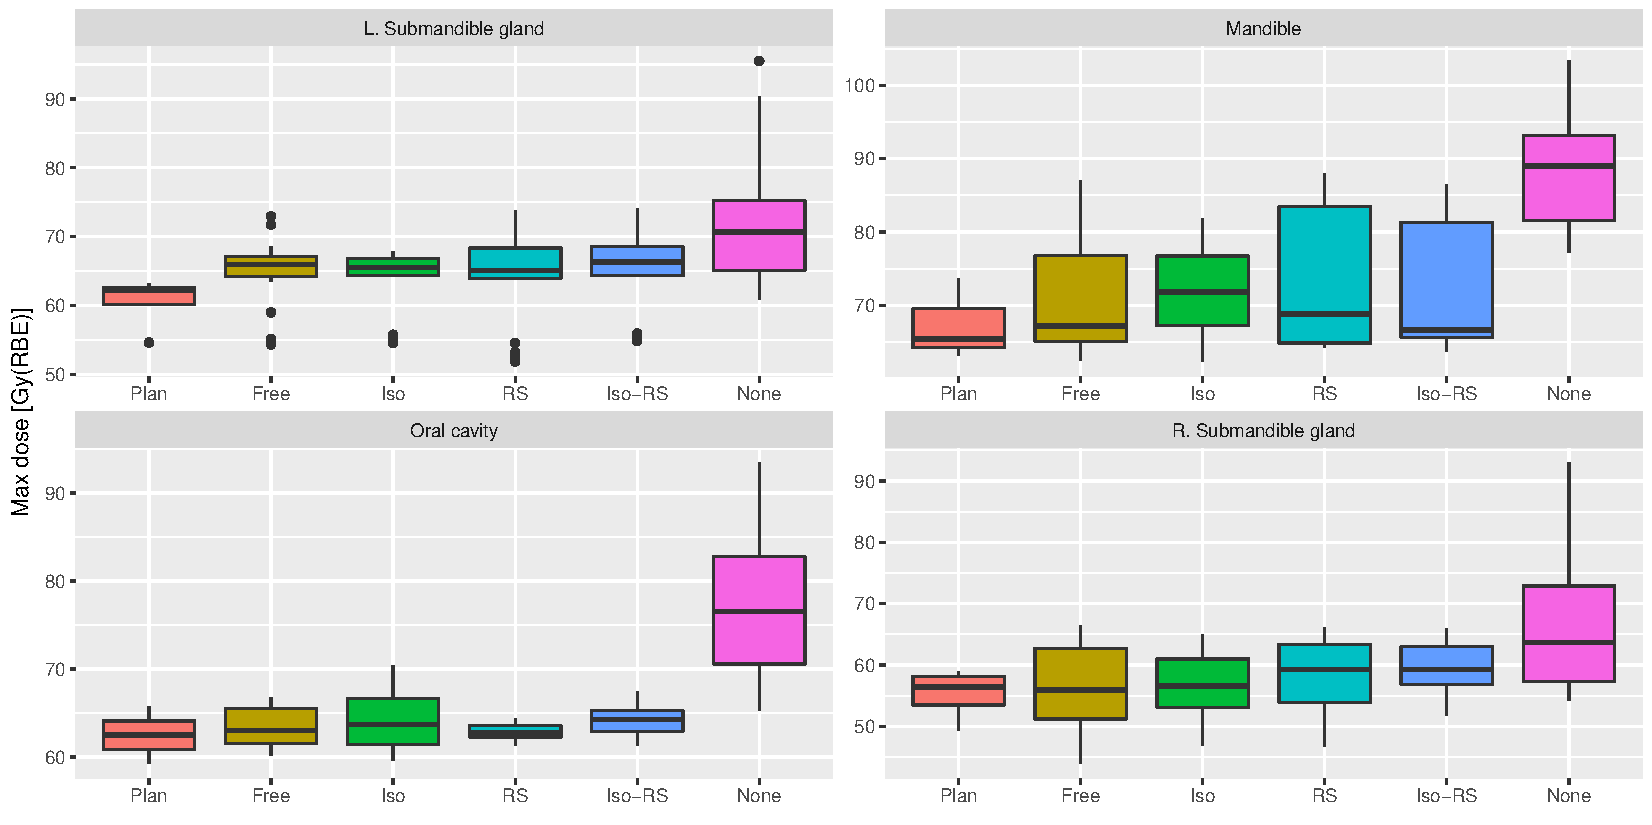
\includegraphics[width=\textwidth]{imgs/oars_max_weights.pdf}}
	\end{figure}
	The DVHs are normalized to V98 = 98\%.
\end{frame}


\begin{frame}[c]{Results overview}
    \only<1>{
    \begin{figure}[h]
        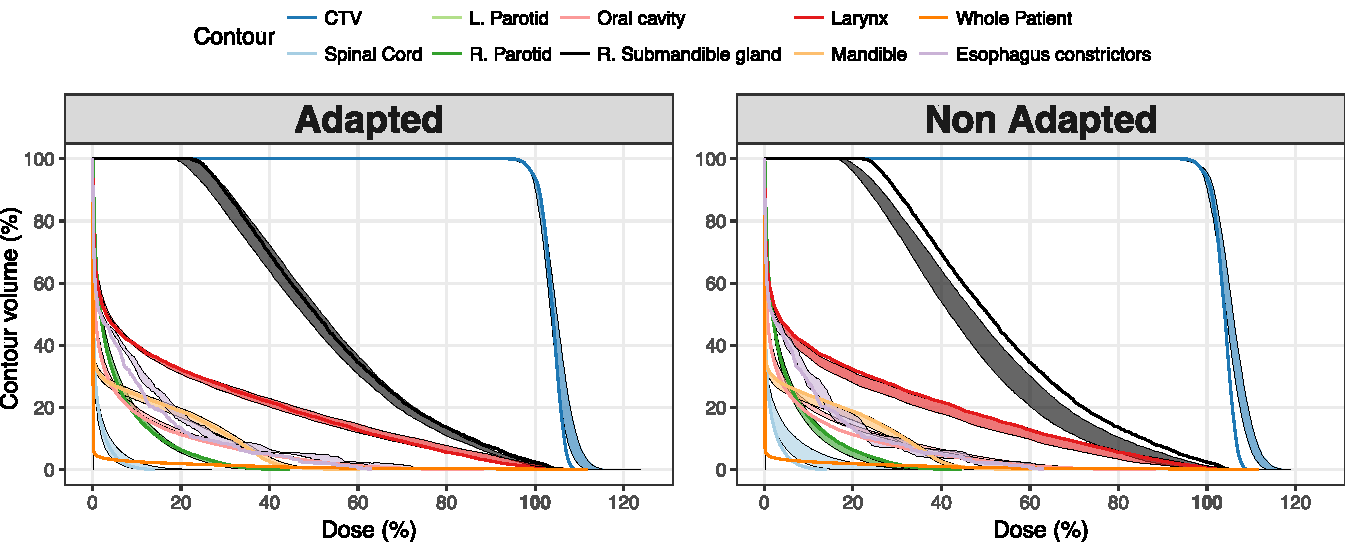
\includegraphics[width=\textwidth]{imgs/DVHs_normalized_Geo_free_P15_not_week6.pdf}
        \caption{Patient 9, adaptation vs plan}
    \end{figure}
    }
    \only<2>{
    \begin{figure}[h]
        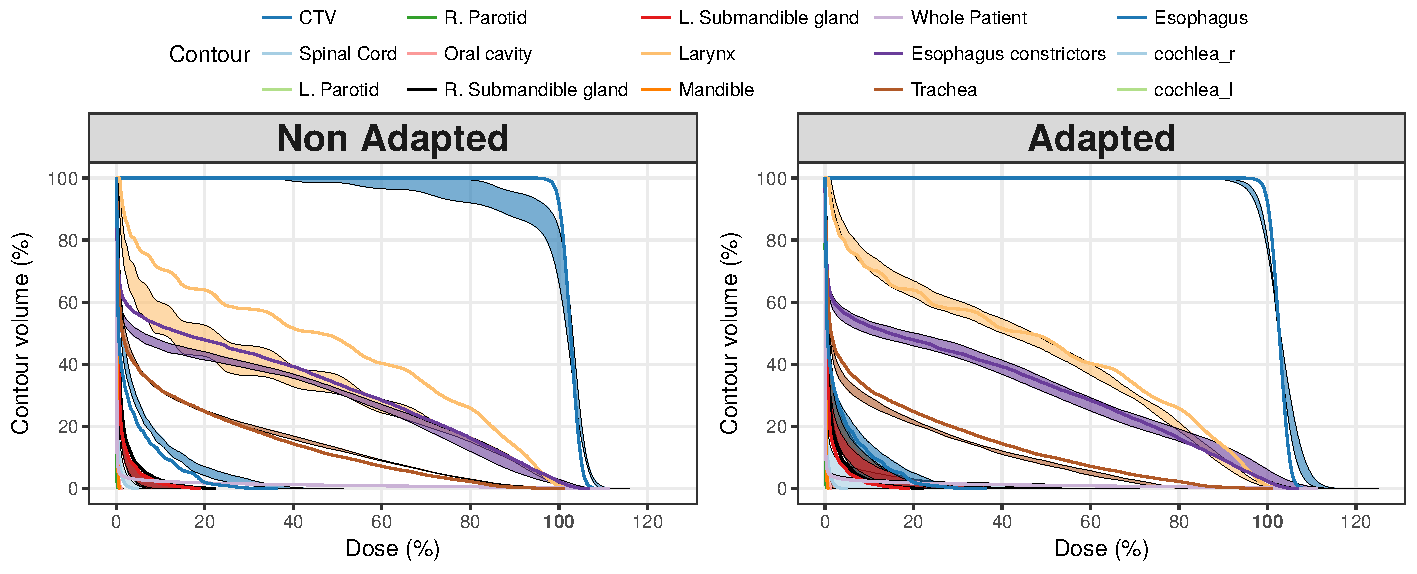
\includegraphics[width=\textwidth]{imgs/DVHs_Weight_Free_P10.pdf}
        \caption{Patient 7, adaptation vs plan}
    \end{figure}
    }
    \only<3>{
    \begin{figure}[h]
        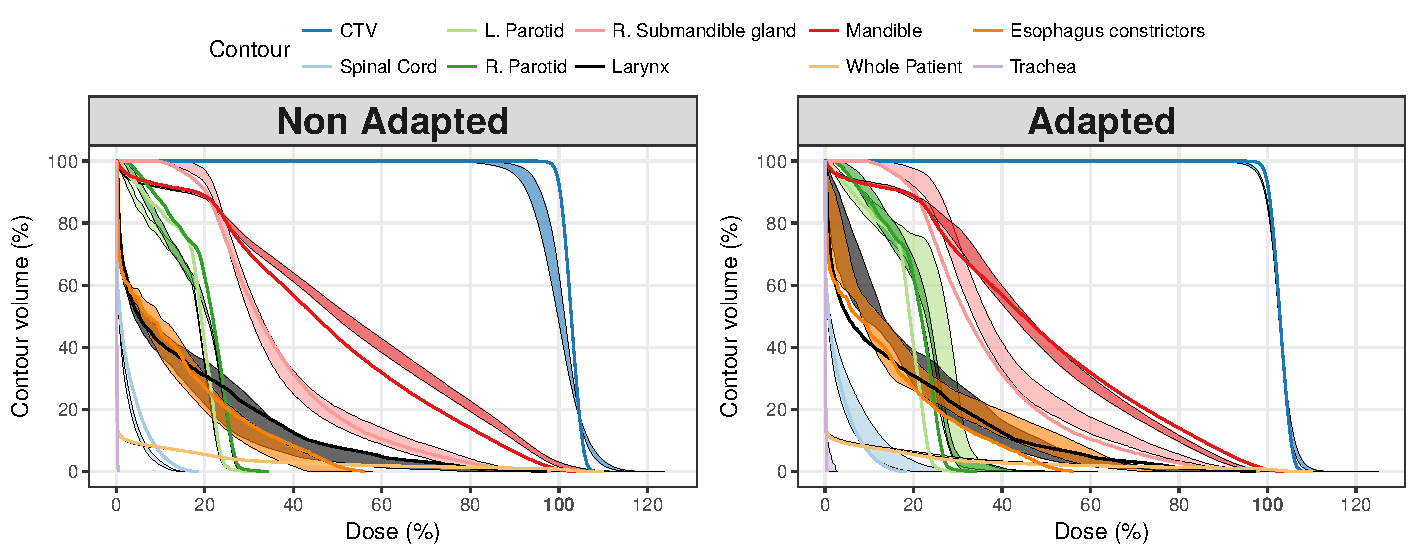
\includegraphics[width=\textwidth]{imgs/DVHs_Weight_Free_P14.pdf}
        \caption{Patient 8, adaptation vs plan}
    \end{figure}
    }
    \only<4>{
    \begin{figure}[h]
        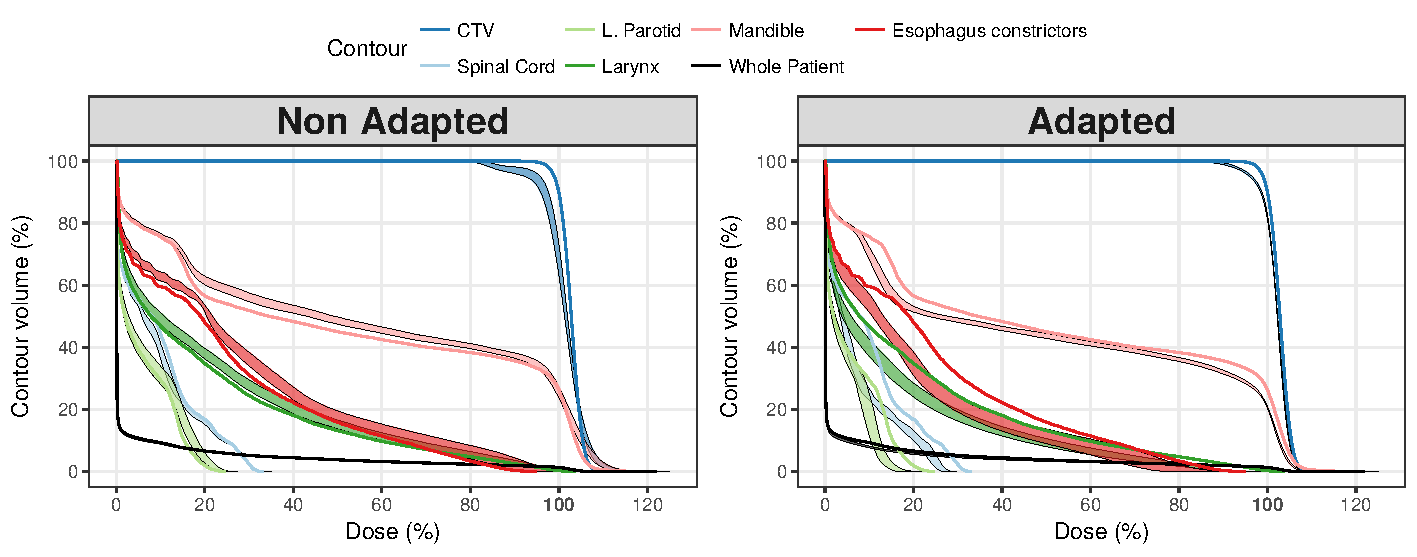
\includegraphics[width=\textwidth]{imgs/DVHs_Weight_Free_P07.pdf}
        \caption{Patient 6, adaptation vs plan}
    \end{figure}
    }
\end{frame}


\begin{frame}[c]{A quick peek into the next studies}
    \begin{figure}[h]
        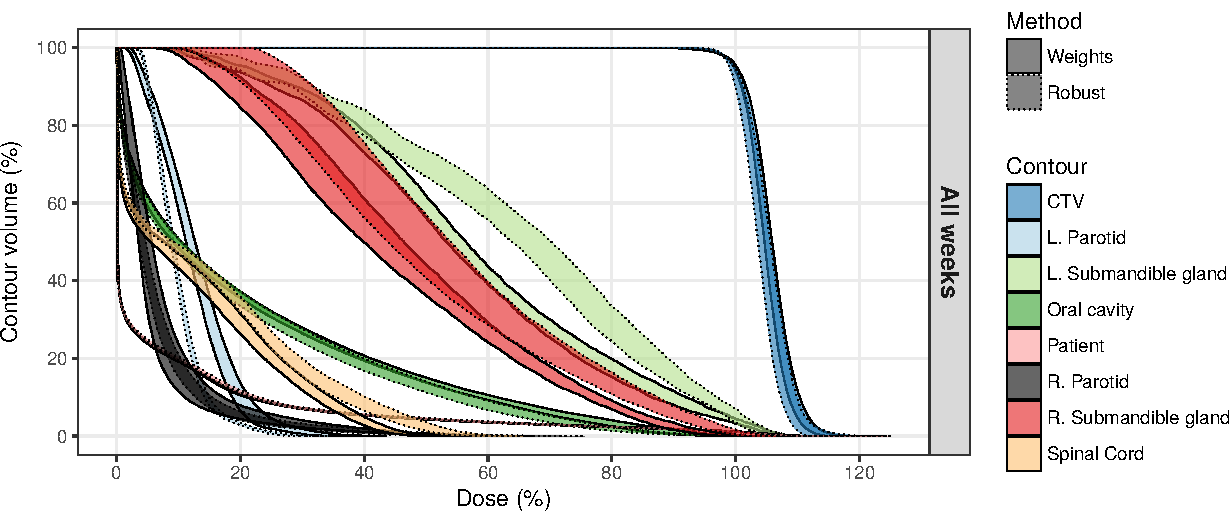
\includegraphics[width=\textwidth]{imgs/robust_opt.pdf}
        \caption{Patient 1, \textbf{adaptation vs ideal robust optimization}}
    \end{figure}
\end{frame}


\begin{frame}[c]{Timing, timing, timing!!}
    \begin{table}[h]
    \scalebox{0.8}{
        \begin{tabular}{l|ccc|c}
             & Minimum & Average & Maximum & Expected \\
            \hline
            Geometrical adapt. & 11.7  & 16.9  & 26.57 & $\sim1-5$ \\
            gPMC validation    & 115.6 & 261.9 & 419.2 & $\sim30$ \\
            Weight tuning      & 12.0  & 44.8  & 198.0 & ?? \\
            \hline
            Total              &   -   & 322.7 &   -   & $\sim60$ \\
            \hline
            $D_{ij}$ size (MB) & 4.1   & 77.9  & 312.0 & 50\% \\
            \hline
        \end{tabular}
        }
        \caption{Current and expected times}
    \end{table}
    Improvements:
    \begin{itemize}
        \item Geometrical adapt.: VF masks, binnings, multithreading\ldots
        \item gPMC validation: Multiple GPUs, unified codes, optimal stopping, kernel occupancy, thread variance reduction\ldots
        \item Opt4D optimization: I am not a great expert, but the dose matrices can be smaller
    \end{itemize}

\end{frame}


\section{Conclusions}
\begin{frame}[c]{Conclusions and outlook}
    Conclusions:
	\begin{itemize}
		\item We have developed and online adaptation algorithm using GPU-MC
		\item The algorithm is able to recover good plan quality
		\item This tool might be useful to allow uncertainty margin reduction
	\end{itemize}
	\pause
	Future work:
    \begin{itemize}
        \item Improve spot selection
        \item Flexible number of particles per spot in gPMC
        \item Compare against robust optimization
        \item Include uncertainties
    \end{itemize}
\end{frame}


\begin{frame}[plain]
    \begin{figure}[h]
        
\includegraphics[width=0.7\textwidth]{imgs/thanks.png}
    \end{figure}
\end{frame}

% \input{05_backup.tex}

\end{document}